\pagebreak
\pagenumbering{Roman}
\section{Anhang}
\subsection{Ergänzende Abbildungen zu Booklet Teil 1}
\label{app:abb_booklet_1}
Folgende Abbildungen stellen die Entscheidungsbäume der Cost-Complexity Aufgabe dar. Der Unterschied in den Bäumen mit geringerem und höherem $\alpha$ wird für die beiden Baum-Variationen gut ersichtlich. Abbildungen \ref{fig:ccp_fulltree_alpha_0005} und \ref{fig:ccp_fulltree_alpha_002} zeigen je einen vollständig ausgebildeten Baum, der durch Cost-Complexity \gqq{beschnitten} wurden.\\
\begin{figure}[H]
	\centering
	\begin{minipage}{0.45\textwidth}
		\centering
		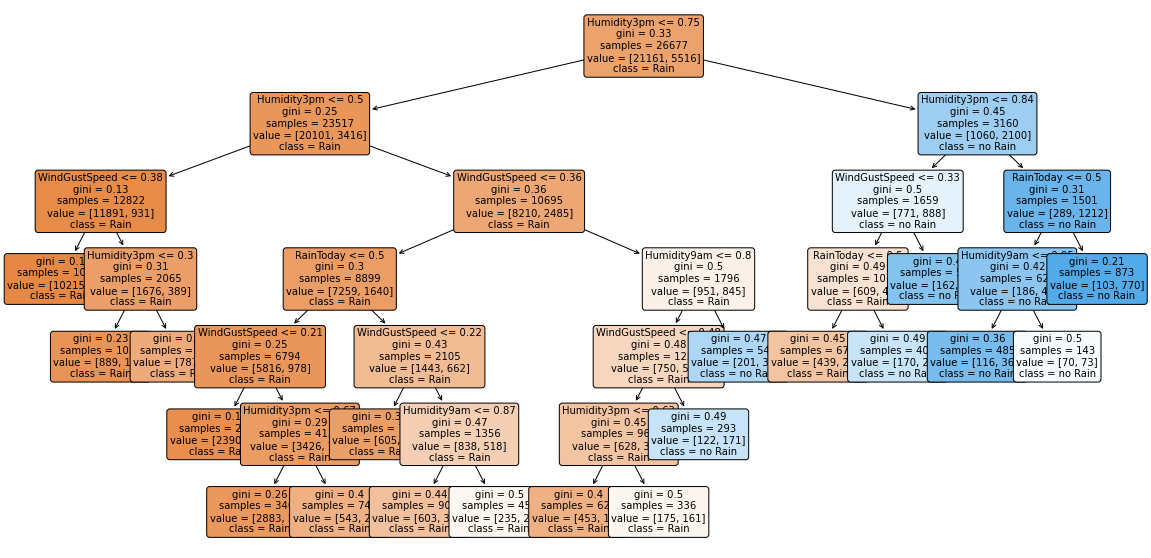
\includegraphics[width=0.9\textwidth]{Bilder/ccp_fulltree_alpha_0005.png}
		\caption{Entscheidungsbaum mit Parametern \emph{max\_depth=None} und \emph{ccp\_alpha=0.0005}}
		\label{fig:ccp_fulltree_alpha_0005}
	\end{minipage}\hfill
	\begin{minipage}{0.45\textwidth}
		\centering
		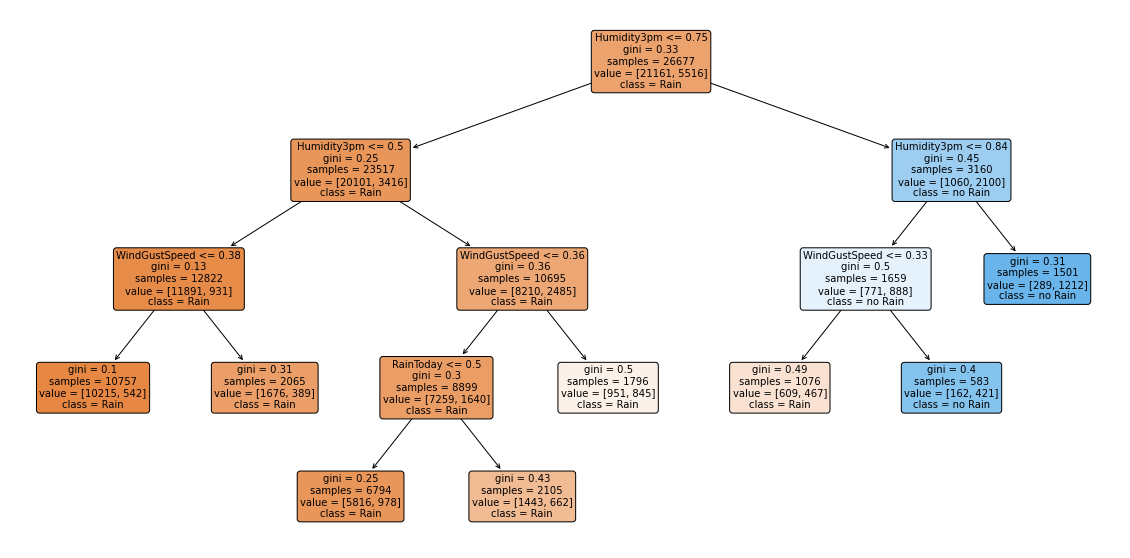
\includegraphics[width=0.9\textwidth]{Bilder/ccp_fulltree_alpha_002.png}
		\caption{Entscheidungsbaum mit Parametern \emph{max\_depth=None} und \emph{ccp\_alpha=0.002}}
		\label{fig:ccp_fulltree_alpha_002}
	\end{minipage}\hfill
\end{figure}
Abbildungen \ref{fig:ccp_maxDepth_alpha_001} und \ref{fig:ccp_maxDepth_alpha_004} zeigen je einen beschnittenen Baum der mit der Einstellung \emph{max\_depth = 8} erstellt wurde.\\
\begin{figure}[H]
	\centering
	\begin{minipage}{0.45\textwidth}
		\centering
		\includegraphics[width=0.9\textwidth]{Bilder/ccp_maxDepth_alpha_001.png}
		\caption{Entscheidungsbaum mit Parametern \emph{max\_depth=8} und \emph{ccp\_alpha=0.001}}
		\label{fig:ccp_maxDepth_alpha_001}
	\end{minipage}\hfill
	\begin{minipage}{0.45\textwidth}
		\centering
		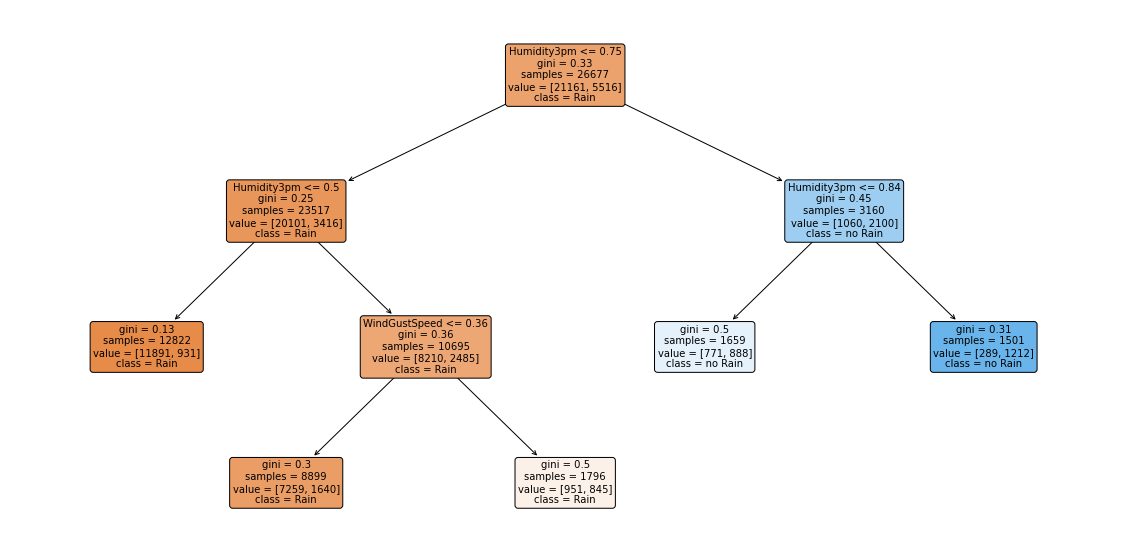
\includegraphics[width=0.9\textwidth]{Bilder/ccp_maxdepth_alpha_004.png}
		\caption{Entscheidungsbaum mit Parametern \emph{max\_depth=8} und \emph{ccp\_alpha=0.004}}
		\label{fig:ccp_maxDepth_alpha_004}
	\end{minipage}\hfill
\end{figure}
\noindent \hspace*{7mm}
Trotz dass der originale Baum ohne Tiefenbegrenzung sehr viel größer ist, als der Baum mit einer maximalen Tiefe von 8, sind die Resultate des Cost-Complexity Prunings ungefähr gleich groß. Die ursprüngliche Größe vor dem Pruning hat somit keinen Einfluss auf das Endergebnis.
\pagebreak
\subsection{Quellcode zu Booklet Teil 1}
\pagebreak
\subsection{Ergänzungen zu Booklet Teil 2} \label{app:ergaenzung_booklet_2}
Als Ergänzung zur Aufgabenstellung und der folgenden mathematischen Herleitung der Backpropagation ist das beschriebene Model in Abbildung \ref{fig:nn_schema} schematisch mit den entsprechenden Variablennamen dargestellt.
\begin{figure}[H]
	\centering
	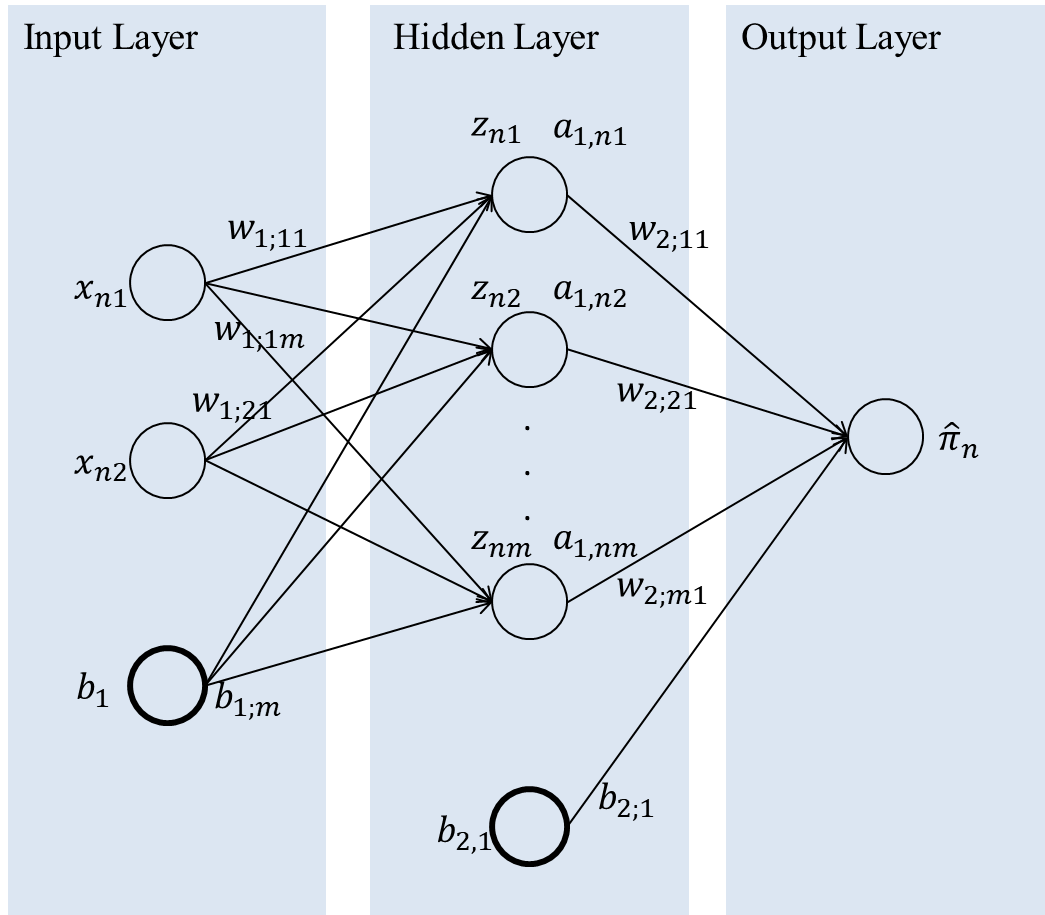
\includegraphics[width = 0.7\textwidth]{Bilder/neuralNetwork.png}
	\caption{Schematische Darstellung des betrachteten Neuronalen Netzes}
	\label{fig:nn_schema}
\end{figure}
y: Beobachtete Werte der Stichprobe\\
$\sigma$ = Sigmoid-Funktion\\
\begin{align*}
dW_{2} &= \frac{\partial E}{\partial W_{2}}\\
&= \frac{\partial E}{\partial z_{2}}\cdot \frac{\partial z_{2}}{\partial W_{2}}\\
&= \frac{\partial E}{\partial \hat{\pi}} \cdot \frac{\partial \hat{\pi}}{\partial z_{2}} \cdot \frac{\partial z_{2}}{\partial W_{2}}\\
&= \frac{\partial }{\partial \hat{\pi}} \frac{1}{2}(y-\hat{\pi}i)^{2} \cdot \frac{\partial }{\partial z_{2}} \sigma(a_{1}W_{2} + b_{2})\cdot \frac{\partial }{\partial W_{2}}(a_{1}W_{2}+b_{2})\\
&= -(y-\hat{\pi}) \cdot \sigma(a_{1}W_{2}+b_{2})(1-\sigma(a_{1}W_{2}+b_{2}))\cdot a_{1}\\
% &= \left[ -\begin{pmatrix}
%     y_{1}  -  a_{2;11} \\
%     \vdots \\
%     y_{n}  -  a_{2;n1}  \\
%     \end{pmatrix} \cdot \begin{pmatrix}
%                         \sigma (z_{2;11}) \\
%                         \vdots \\
%                         \sigma (z_{2;n1})  \\
%                         \end{pmatrix} \cdot \begin{pmatrix}
%                                                 1-\sigma (z_{2;11}) \\
%                                                 \vdots \\
%                                                 1-\sigma (z_{2;n1})  \\
%                                                 \end{pmatrix}\right]^{T} \cdot \begin{pmatrix}
%                                                                     a_{1;11} & \cdots & a_{1;1m} \\
%                                                                     \vdots & \ddots & \vdots \\
%                                                                     a_{1;n1}&\cdots & a_{1;nm}  \\
%                                                                     \end{pmatrix}\\\\
\Rightarrow \delta_{2} &= \frac{\partial E}{\partial z_{2}}\\
\delta_{2} &= -(y-\hat{\pi}) \cdot \sigma(a_{1}W_{2}+b_{2})(1-\sigma(a_{1}W_{2}+b_{2}))\\\\
db_{2} &= \frac{\partial E}{\partial b_{2}}\\
&=\frac{\partial E}{\partial z_{2}} \cdot \frac{\partial z_{2}}{\partial b_{2}}\\
&= \frac{\partial E}{\partial\hat{\pi}} \cdot \frac{\partial \hat{\pi}}{\partial z_{2}} \cdot \frac{\partial z_{2}}{\partial b_{2}}\\
&= \delta_{2} \cdot 1\\
&= -(y-\hat{\pi}) \cdot \sigma(a_{1}W_{2}+b_{2})(1-\sigma(a_{1}W_{2}+b_{2})) \cdot 1\\\\
% &=\left[-\begin{pmatrix}
%     y_{1}  -  a_{2;11} \\
%     \vdots \\
%     y_{n}  -  a_{2;n1}  \\
%     \end{pmatrix} \cdot \begin{pmatrix}
%                         \sigma (z_{2;11}) \\
%                         \vdots \\
%                         \sigma (z_{2;n1})  \\
%                         \end{pmatrix} \cdot \begin{pmatrix}
%                                                 1-\sigma (z_{2;11}) \\
%                                                 \vdots \\
%                                                 1-\sigma (z_{2;n1})  \\
%                                                 \end{pmatrix}\right]^{T} \cdot \begin{pmatrix}
%                                                                         1 \\
%                                                                         \vdots \\
%                                                                         1  \\
%                                                                         \end{pmatrix} \\\\
dW_{1} &= \frac{\partial E}{\partial W_{1}}\\
&= \delta_{1} \cdot X
\end{align*}
\begin{align*}    
\Rightarrow \delta_{1} &= \frac{E}{\partial z_{1}}\\
&= \sum_{k=1}^{1} \frac{\partial E}{\partial z_{2}}\cdot \frac{\partial z_{2}}{\partial z_{1}}\\
&=  \delta_{2} \cdot \frac{\partial z_{2}}{\partial z_{1}}\\
&=  \delta_{2}\cdot \frac{\partial }{\partial a_{1}}(a_{1}W_{2}+b_{2})\cdot \frac{\partial }{\partial z_{1}}\sigma(X\cdot W_{1} +b_{1})\\
&=  \delta_{2}\cdot W_{2} \cdot \sigma(X\cdot W_{1}+b_{1})(1- \sigma(X\cdot W_{1}+b_{1}))\\
% \Rightarrow dW_{1}&= \delta_{2} \cdot \begin{pmatrix}
%                     w_{2;11} \\
%                     \vdots \\
%                     w_{2;m1} \\
%                     \end{pmatrix} \cdot \begin{pmatrix}
%                                         \sigma (z_{1;11})& \cdots & \sigma(z_{1;1m}) \\
%                                         \vdots & \ddots &\vdots\\
%                                         \sigma (z_{1;n1}) & \cdots & \sigma (z_{1;nm})  \\
%                                         \end{pmatrix} \cdot \begin{pmatrix}
%                                                             1-\sigma (z_{2;11}) \\
%                                                             \vdots \\
%                                                             1-\sigma (z_{2;n1})  \\
%                                                             \end{pmatrix} \cdot \begin{pmatrix}
%                                                                                      x_{11} & x_{12}\\
%                                                                                      \vdots & \vdots\\
%                                                                                      x_{n1} & x_{n2}\\
%                                                                                     \end{pmatrix} \\\\
\end{align*}
Bemerkung zu $\delta_{1}$: der Parameter $k$ entspricht der Anzahl an Knoten im Output Layer. Da das betrachtete Modell nur einen Knoten im Output Layer besitzt, kann diese Summe weggelassen werden, da es nur einen Summanden gibt.
\begin{align*} 
db_{1} &= \delta_{1} \cdot \frac{\partial}{\partial b_{1}}\sigma(X\cdot W_{1}+b_{1})\\
&= \delta_{1} \cdot 1\\
% &= \delta_{2} \cdot \begin{pmatrix}
%                     w_{2;11} \\
%                     \vdots \\
%                     w_{2;m1} \\
%                     \end{pmatrix} \cdot \begin{pmatrix}
%                                         \sigma (z_{1;11})& \cdots & \sigma(z_{1;1m}) \\
%                                         \vdots & \ddots &\vdots\\
%                                         \sigma (z_{1;n1}) & \cdots & \sigma (z_{1;nm})  \\
%                                         \end{pmatrix} \cdot \begin{pmatrix}
%                                                             1-\sigma (z_{2;11}) \\
%                                                             \vdots \\
%                                                             1-\sigma (z_{2;n1})  \\
%                                                             \end{pmatrix} \cdot 1
\end{align*}
\subsection{Quellcode zu Booklet Teil 2} \label{app:quellcode_booklet_2}
\pagebreak
\subsection{Ergänzende Tabellen zu Teil 3} \label{app:3_ergaenzungen}

\begin{table}[H]
	\centering
	\begin{tabular}{ll}
		\hline
		Hyperparameter              & Parameterraum                              \\ \hline
		n\_estimators               & {[}10, 50, 100{]}                          \\
		criterion                   & {[}gini, entropy{]}                    \\
		max\_depth                  & {[}None, 3,5,10, 15, 20, 25, 50{]}         \\
		min\_samples\_split         & {[}2, 5,10, 20, 30, 40{]}                  \\
		min\_samples\_leaf          & {[}1, 2, 5, 10, 20, 40, 100, 200{]}                  \\
		min\_weight\_fraction\_leaf & {[}0, 0.2, 0.4, 0.5{]}                     \\
		max\_features               & {[}None, 5, 10, 15 ,20, 25{]}              \\
		max\_leaf\_nodes            & {[}None, 2 ,10, 100, 150, 200, 300, 500{]} \\
		min\_impurity\_decrease     & {[}0.0, 0.001, 0.002, 0.01, 0.1{]}     \\
		min\_impurity\_split        & {[}0.0, 0.1, 0.2, 0.5, 0.8, 1, 2, 3{]}     \\ \hline
	\end{tabular}
	\caption{Parameterräume der univariaten \emph{Grid Search}}
	\label{table:parameter_grid_univariat}
\end{table}

\begin{table}[H]
	\centering
	\begin{tabular}{lll}
		\hline
		Hyperparameter          & Parameterraum                       & Gewählter Parameter \\ \hline
		max\_depth              & {[}None, 5, 10, 15{]}               & None                \\
		min\_samples\_split     & {[}2, 5, 10{]}                      & 5                   \\
		max\_features           & {[}None, 5, 20, 25{]}               & None                \\
		min\_impurity\_decrease & {[}0.00005, 0.0001, 0.001, 0.003{]} & 0.00005             \\ 
		n\_estimators &  & 100 \\ \hline
	\end{tabular}
	\caption{\label{table:parameter_grid_multivariat_forest} Parameterräume und Ergebnisse der multivariaten \emph{Grid Search} des Random Forest}
\end{table}


\begin{table}[H]
	\centering
	\begin{tabular}{lll}
		\hline
		Hyperparameter          & Parameterraum                       & Gewählter Parameter \\ \hline
		max\_depth              & {[}None, 5, 10, 15{]}               & None                \\
		min\_samples\_split     & {[}2, 5, 10{]}                      & 5                   \\
		max\_features           & {[}None, 5, 20, 25{]}               & None                \\
		min\_impurity\_decrease & {[}0.00005, 0.0001, 0.001, 0.003{]} & 0.00001             \\ \hline
	\end{tabular}
	\caption{\label{table:parameter_grid_multivariat_tree} Parameterräume und Ergebnisse der multivariaten \emph{Grid Search} des Entscheidungsbaums}
\end{table}

\begin{table}[H]
	\centering
	\begin{tabular}{lll}
		\hline
		Hyperparameter          & Parameterraum                        & Gewählter Parameter \\ \hline
		max\_depth              & {[}None, 5, 10, 20. 25{]}                & 20                   \\
		min\_samples\_split     & {[}2, 5, 10, 20{]}                   & 2                  \\
		max\_features           & {[}None, 5, 20, 25{]}                & None                  \\
		min\_impurity\_decrease & {[}0.0, 0.0001, 0.0005, 0.001{]} & 0.0             \\ 
		n\_estimators &  & 100 \\ \hline
	\end{tabular}
	\caption{\label{table:parameter_grid_multivariat_adaboost} Parameterräume und Ergebnisse der multivariaten \emph{Grid Search} des Adaboost-Verfahrens}
\end{table}

\begin{table}[H]
	\centering
	\begin{tabular}{lll}
		\hline
		Hyperparameter          & Parameterraum                        & Gewählter Parameter \\ \hline
		max\_depth              & {[}None, 5, 10, 15{]}                & None                \\
		min\_samples\_split     & {[}2, 5, 10, 20{]}                   & 10                  \\
		max\_features           & {[}None, 5, 20, 25{]}                & 5                   \\
		min\_impurity\_decrease & {[}0.00005, 0.0001, 0.0005, 0.001{]} & 0.0001              \\ 
		n\_estimators &  & 100 \\ \hline
	\end{tabular}
	\caption{\label{table:parameter_grid_multivariat_bagging} Parameterräume und Ergebnisse der multivariaten \emph{Grid Search} des Bagging-Verfahrens}
\end{table}
\subsection{Quellcode zu Booklet Teil 3}

\pagebreak
\subsection{Ergänzungen zu Booklet Teil 4}\label{app:svm_ergaenzungen}
Abbildung \ref{fig:svm_2d} zeigt einen zweidimensionalen \emph{Input Space} dessen Daten durch Transformation in einem dreidimensionalen \emph{Feature Space} linear trennbar sind (s. Abbildung \ref{fig:svm_3d})\\
\begin{figure}[h]
	\centering
	\subfloat[zwei-dimensionaler Input-Space]{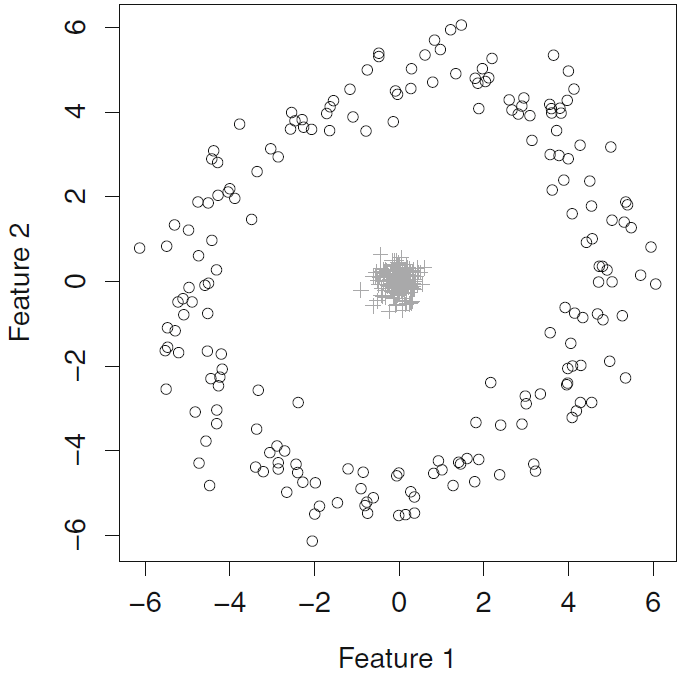
\includegraphics[width=0.40\textwidth]{Bilder/svm_2d.png}\label{fig:svm_2d}}
	\hfill
	\subfloat[drei-dimensionaler Feature-Space]{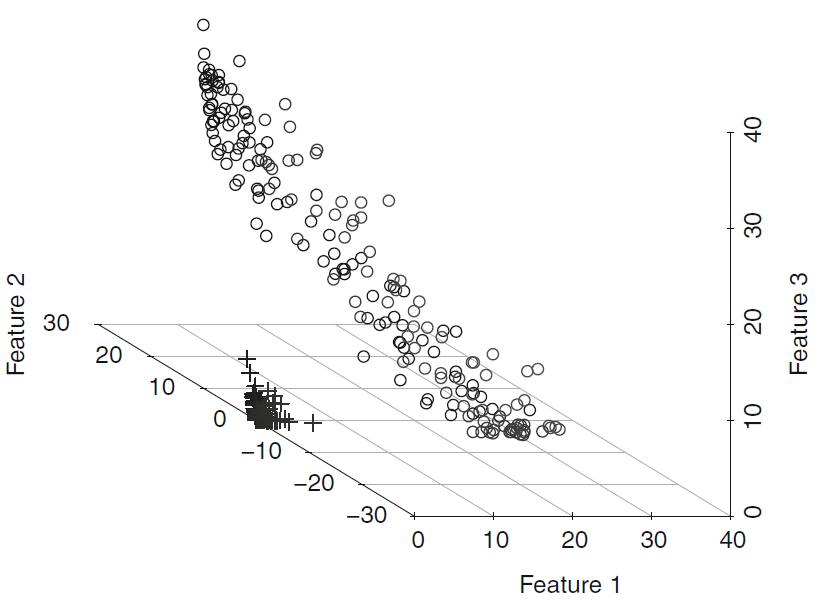
\includegraphics[width=0.40\textwidth]{Bilder/svm_3d.png}\label{fig:svm_3d}}
	\caption{Transformation der Daten durch Kernfuntionen (\cite{2018_mello_ponti})}
\end{figure}
Tabelle \ref{tab:svm_results_gridSearch} zeigt die genauen Parameterräume, die wurch das \emph{Grid Search} Verfahren untersucht wurden. Zudem sieht man für jeden Kernel die besten Parameter und die Genauigkeit des trainierten Modells. Der Kerneltyp \emph{precomputed} wurde hierbei nicht beachtet.
\begin{table}[H]
	\begin{tabular}{lllll}
		\hline
		Kernel& Parameterräume & Parameterergebnisse & Accuracy \\ \hline
		Linear &  C: [0.1, 1.0, 10.0, 100.0]  &  C: 1.0      &  0.85047   \\ \hline
		Polynomial  &  C: [0.1, 1.0, 10.0, 100.0] & C: 1.0     &  0.86153   \\
		&  coef0: [0, 0.5, 1.0] & coef0: 1.0    &     \\
		&  degree: [2.0, 3.0, 4.0, 5.0] &degree:  4.0   &      \\
		&  gamma: ['scale', 'auto', 0.01, 1.0] & gamma: 'scale'    &      \\\hline
		RBF &  C: [0.1, 1.0, 10.0, 100.0]  &   C: 10.0    &   0.86198   \\
		&  gamma: ['scale', 'auto', 0.01, 1.0] &   gamma: 'scale'   &    \\ \hline
		Sigmoid&  C: [0.1, 1.0, 10.0, 100.0] &   C: 10.0   &  0.85028  \\
		&  gamma: ['scale', 'auto', 0.01, 1.0] &  gamma: 0.01   &   \\
		&  coef0: [0.0, 0.5, 1.0] &  coef0: 0.0   &   \\ \hline
	\end{tabular}
	\caption{ Parameterräume und Ergebnisse der Grid Search}
	\label{tab:svm_results_gridSearch}
\end{table}

\subsection{Quellcode zu Booklet Teil 4}